\chapter{Introduction to data}
\label{introductionToData}


\setcounter{section}{4}

%%%%%
\section{Basic data collection}
\label{basicDataCollection}

The first step in conducting research is to identify topics or questions that are to be investigated. A clearly laid out research question is helpful in identifying what subjects or cases are to be studied and what variables are important. This information provides a foundation for \emph{what} data will be helpful. It is also important that we consider \emph{how} data is collected so that it is trustworthy and helps achieve the research goals. This section outlines important ideas and practices in data collection. %not only lays the groundwork for what data should be collected for research questions but also how to collect that data. This information is also helpful in evaluating the integrity of data collected by others.

%It is important to identify what information will most efficiently and accurately answer research questions prior to collecting data. To do so, the research questions that we hope to answer.

%\Comment{Describe components of the research question and how they influence what data to collect and how much to collect.}

%\Comment{Then we move onto data quality or ``trustworthy data and to judge the quality of data produced by others... careful design of data production is the most important prerequisite for trustworthy inference.'' (Moore \& McCabe, p192).}

%\subsection{Getting started}

%\Comment{First step is to identify both who/what is to be studied. This means identifying what people or things are to be sampled, and what data is to be collected about each case. Emphasize that this may be a difficult task and requires careful considerations. (MM192)}

%Here we consider two research questions important to many college students:
%\begin{itemize}
%\item Do folks who have a graduate degree earn more than those folks who without a graduate degree?
%\item Would a person maximize her income by obtaining a graduate degree or having additional outside experience?
%\end{itemize}
%These questions are similar in that they ask about the same variables: graduate education and income. However, the first only asks about what we observe in the population. The second asks what would happen under two different circumstances. To answer each question

%\subsection{Identifying an appropriate study method}

%Do folks who have college degree tend to make more money than folks who don't have a college degree? The research question considered here can be categorized as a \emph{What is?} question, and it can be answered by examining demographic data. Below are the average incomes for folks with and without a college degree in 2008:
%\begin{tabbing}
%\hspace{\parindent}  \= With a college degree: \=\hspace{8mm}\= \$ \\
%				\> Without a college degree: \>\>		    \$ \\
%\end{tabbing}
%\addvspace{-5mm}
%For people in the US, we can conclude that yes, folks with a college degree make more money on the average.

%We might ask a more interesting question: Is it more wise to pursue a college degree if the sole goal is to increase salary? After all, an additional four years of experience may be more valuable. Here we are asking a \emph{What if?} question. Would a person tend to do better or worse financially if she pursued a college degree? A first thought might be to say ``Yes, because look at the population data.'' However, perhaps it is not the college degree that actually caused those folks to have more money. Perhaps they would have even more money had they not gone to college. There is no way to answer this \emph{What if?} question using the summary statistics listed above.


% This is a much more difficult and complex question. The answer may be different from one individual to another individual,  also varies from one person to the other.

% What if the education of the same folks was actually different? Would we still observe the same set of folks, irregardless of their college education, averaging a higher income? Here we want to answer a were modified? What if a person had a chance to who had a college degree was able to go back in time and choose a different path?




%When we make a research question, it typically takes one of two forms:
%\begin{itemize}
%\item \textbf{What is?} Here we are interested in the current status or existing relationship between certain variables. Do folks who have college degree tend to have more money than folks who don't have a college degree? That is, is there an association between a person having a college degree and her net wealth?
%\item \textbf{What if?} When we ask \emph{What if?} we wonder, if we adjust one variable, does it affect the other? For instance, would a group of folks typically make more money if they earned a graduate degree than if they had not earned a graduate degree? Here we are not asking \emph{What is?} and instead are asking \emph{What if?}. % While this again asks about some connection between higher education and income, this research question runs deeper: is there a \emph{causal} connection between education and income?
%\end{itemize}
%When we ask a \emph{What is?} question, we are wondering whether two or more variables are naturally associated. %When we ask a \emph{What if?} question, we wonder whether one variable 


%Consider the following two research questions:
%\begin{itemize}
%\item If someone owns a Toyota vehicle, is she less likely to die from a heart attack?
%\item Are folks who take a daily aspirin less likely to die from a heart attack?
%\end{itemize}

% If we wanted to identify the exact  Here, a case represents a student who has enrolled in UCLA's undergraduate program. The population of interest is all students who have enrolled in UCLA's undergraduate program and have finished.

%Many research questions ask about the status of the world or to summarize characteristics of \emph{what is}.

%\Comment{Identifying the population or process of interest.}\\


%When we make a research question, we often try to answer it typically takes two forms:
%\begin{itemize}
%\item \textbf{What is?} Here we are interested in the current status or existing relationship between certain variables. For example, are folks who take a daily aspirin less likely to die from a heart attack? % folks with more education make more money? We collect \emph{observational data} to answer such questions. %are male or female possums longer, on average? These types of research questions about the \emph{natural order} of the world can be answered by collecting data from cases in some population. To determine if male or female possums are longer, we could collected a sample of possums from the population of all possums.
%\item \textbf{What if?} If turn a crank here, what happens over there? If a person  Does providing more education to a group of folks tend to cause an increase in their future income? To analyze such questions, we
%For instance, what if we gave heart-attack patients a new drug? Would it reduce their chance of death? In these types of questions, we would like to make some \emph{causal} connection. To provide convincing data that such a causal relationship exists, we must conduct an \emph{experiment}.
%\end{itemize}
%These two types of research questions are best answered by their own respective data collection technique.

%When we ask \emph{What is?}, we are often asking about connections between variables.

\subsection{Populations and samples}
\label{populationsAndSamples}

Consider the following three research questions:
\begin{enumerate}
\item What is the average mercury content in swordfish in the Atlantic Ocean?
\item\label{timeToGraduationQuestionForUCLAStudents} Over the last 5 years, what is the average time to degree for UCLA undergraduate students?
%how long has it taken students to complete their Ba
%How long does it take a student to complete a Bachelor's degree at your university? That is, what is the average time to degree?
%\item Of those students who graduate,  is the typical time to graduation for undergraduate students at UCLA? That is, what is the average number of years it takes a student at UCLA to earn her undergraduate degree?
%\item\label{textbooksAtAmazonOrSchoolPopulationQuestion} Are textbooks used in university classes typically cheaper on Amazon.com or at university bookstores?
%\item What is the average income of students who have graduated from my high school who did not go to college?
\item\label{identifyPopulationOfSulphinpyrazone} Does the drug sulphinpyrazone reduce the number of deaths in heart attack patients?
\end{enumerate}
In each research question, some population of cases is considered. In the first question, all swordfish in the Atlantic ocean are relevant to answering the question. Each fish represents a case, and all of these fish represent the \term{population} of cases. Often times, it is too expensive to collect data for every case in a population. Instead a \emph{sample} is taken of the population. A \term{sample} represents a subset of the cases and often times represents only a small fraction of all cases in the population. For instance, 60 swordfish (or some other number) in the population might be selected, and this sample data may be used to provide an estimate of the population average, i.e. an answer to the research question.

\begin{exercise} \label{identifyingThePopulationForTwoQuestionsInPopAndSampSubsection}
For the second and third questions above, identify what is an individual case and also what is the population under consideration. Answers in the footnote\footnote{(\ref{timeToGraduationQuestionForUCLAStudents}) First, notice that this question is only relevant to students who complete their degree; the average cannot be computed using a student who never finished her degree. Thus, only UCLA undergraduate students who have graduated in the last five years represent cases in the population under consideration. (\ref{identifyPopulationOfSulphinpyrazone}) A heart attack patient represents a case. The population represents all heart attack patients.}.
\end{exercise}


\subsection{Anecdotal evidence}

%\begin{quote}
%\emph{I can't believe Nixon won. I don't know anybody who voted for him.}
%\end{quote}

%\Comment{Find three examples where we might draw conclusions based on single events. MM examples: AIDS in young people must be common since we hear so much about it, flying seems more dangerous than driving because airplane crashes stick out in our minds, } \\

%\Comment{``Anecdotal evidence: Anecdotal evidence is based on haphazardly selected individual cases, which often come to our attention because they are striking in some way. These cases need not be representative of any larger group of cases.'' (MM193)} \\

We posed three research questions in Section~\ref{populationsAndSamples}. Below are some statements by folks who are responding to the research questions: % and conclusions based on those observations:
\begin{enumerate}
\item A man on the news got mercury poisoning from eating swordfish, so the average mercury concentration in swordfish must be dangerously high.
\item\label{iKnowThreeStudentsWhoTookMoreThan10YearsToGraduateAtUCLA} I met two students who took more than 10 years to graduate from UCLA, so it must take longer to graduate at UCLA than at many other colleges. %at least 8 years on average to graduate.
\item\label{myFriendsDadDiedAfterSulphinpyrazon} My friend's dad had a heart attack and died after they gave him sulphinpyrazone. The drug must not work.
\end{enumerate}
Each of the conclusions made are based on some data. However, there are two problems. First, the data described only represents a one or two cases. Second and more importantly, it is unclear whether these cases are actually representative of the population. Data collected in this haphazard fashion is called \term{anecdotal evidence}.

\begin{figure}
\begin{centering}
\includegraphics[width=60mm]{01/figures/mnWinter/mnWinter}\hspace{4mm}
\begin{minipage}[b]{\textwidth - 64mm}
%The media regularly reports on striking stories that represent anecdotal evidence. 
\caption[anecdotal evidence]{In February 2010, some media pundits cited one large snow storm as valid evidence against global warming. As comedian Jon Stewart pointed out, ``It's one storm, in one region, of one country.''\footnote{www.openintro.org/clip/anecdotal.php}}%$^{\text{\fnsymbol{alwaysTwo}}}$}
%\footnote{http://www.thedailyshow.com/watch/wed-february-10-2010/unusually-large-snowstorm}}
%. \emph{TIME} reported a story with the headline \emph{Another Blizzard: What Happened to Global Warming?} However, the article actually explained took a reasonable position.)} %one web blog reported \emph{Washington DC covered in snow proves global warming wrong}.} %some television pundits cited unusually cold weather in the Northeast as strong evidence against the validity of global warming. Had they taken a Globally that same winter was the warmest on record (!).} % In a similar vein, a severe summer heat wave is sometimes cited as convincing evidence that global warming is real. }
\label{mnWinter}
\end{minipage}
\end{centering}
%\vspace{1mm}
%\rule{2in}{0.4pt} \\
%\footnotesize $^{\text{\fnsymbol{alwaysTwo}}}$http://www.thedailyshow.com/watch/wed-february-10-2010/unusually-large-snowstorm
\end{figure}


\begin{termBox}{\tBoxTitle{Anecdotal evidence}
Data collected in a haphazard fashion. Such evidence may be true and verifiable but often times represent extraordinary cases.}
\end{termBox}
%\begin{enumerate}
%\item 
%\end{enumerate}

% Additionally, each conclusion is based on only a few observations. 

Anecdotal evidence typically is composed of unusual cases that we recall based on their striking characteristics. For instance, we are more likely to remember the two folks we met who took 10 years to graduate than the six others who graduated in four years. %\\

%\begin{exercise}
%What is a conclusion you or someone you know has come to based on anecdotal evidence? Why did the data stick out in your mind?
%\end{exercise}

%\begin{exercise}
%Explain why the anecdotal cases described above in (\ref{myTextbooksAreMoreExpensiveOnAmazon}) and (\ref{myFriendsDadDiedAfterSulphinpyrazon}) are not necessarily representative of the populations you described in Exercise~\ref{identifyingThePopulationForTwoQuestionsInPopAndSampSubsection}. Answers in the footnote\footnote{(\ref{myTextbooksAreMoreExpensiveOnAmazon}) Maybe all English textbooks are cheaper at the UCLA Bookstore but the reverse is true of all other books. This small sample may not be representative of the population considered. (\ref{myFriendsDadDiedAfterSulphinpyrazon}) Such an emotional experience is easy to recall but may not be representative.}.
%\end{exercise}

Instead of looking at the most unusual cases, we often want to look at a sample that is representative of the population. It is also helpful to collect a sample with many cases.

\subsection{Sampling from a population}

The \data{cars} data set represents a {sample} of cars from 1993. All cars from 1993 represent the {population}, and the cars in the sample were \term{randomly} selected from the population. Randomly selected in this context is equivalent to how raffles are run. The name of each car from the population was written on a raffle ticket, and 54 tickets were drawn.
\begin{figure}
\centering
\includegraphics[height=1.5in]{01/figures/popToSample/popToSample}
\caption{Cars from the population are randomly selected to be included in the sample.}
\label{popToSample}
\end{figure}

Why pick a sample randomly? Why not just pick a sample by hand? Consider the following scenario.

\begin{exercise}
Suppose a muscle car enthusiast is asked to select several cars for a study. What kind of cars do you think she might collect? Do you think her sample would be representative of all cars? %(b) Suppose you realize she might pick cars that reflect her taste if you ask her to pick cars that are representative of all cars? 
\end{exercise}

%Exercise~\ref{} suggests folks might not be very good at picking a representative sample. Even if a person tries very hard to pick a sample representing the population, she might neglect some component that is important.

Even If someone was permitted to pick and choose exactly which cars were included in the sample, it is entirely possible that the sample could be skewed to that person's interests, which may be entirely unintentional. This introduces \term{bias} into a sample. Sampling randomly helps resolve this problem. The most basic random sample is called a \term{simple random sample}, and is the equivalent of using a raffle to select cases. This means that each case in the population has an equal chance of being included and there is no implied connection between the cases in the sample. The act of taking a simple random sample helps eliminate bias, however, it can still crop up in other ways.
\begin{figure}
\centering
\includegraphics[height=1.5in]{01/figures/popToSample/popToSubSample}
\caption{Instead of sampling from all cars from 1993, an environmentalist might inadvertently pick cars with high mileage disproportionally often.}
\label{popToSubSample}
\end{figure}

Even when people are seemingly picked at random (for surveys, etc.), caution must be exercised if the \term{non-response} is high. For instance, if only 15\% of the people randomly sampled for a survey actually respond, then it is unclear whether the results are \term{representative} of the entire population. \term{Non-response bias} can skew results one way or another. %\footnote{In respected polling outfits such as Gallup, researchers try to keep the non-response level low while also making corrections to attempt to offset any lingering bias. These types of corrections are beyond the scope of this text.}.
\begin{figure}[h]
\centering
\includegraphics[height=1.5in]{01/figures/popToSample/surveySample}
\caption{Surveys may result in only reaching a certain group within the population, and it is not obvious how to fix this problem.}
\label{surveySample}
\end{figure}

Another common downfall is a \term{convenience sample}, where individuals who are easily accessible are more likely to be included in the sample. For instance, if a political survey is done by stopping people walking in the Bronx, this probably will not fairly represent all of New York City. It is often difficult to discern what sub-population a convenience sample represents.

\begin{exercise}
We can easily access ratings for products, sellers, and companies through websites. These ratings are based only on those people who go out of their way to provide a rating. If a seller has a rating of 95\% on Amazon, do you think this number might be artificially low or high? %\footnote{For your consideration, one of the authors of this book has sold 67 items on Amazon and only received 16 ratings based on these transactions.}?
Why?
%If you stand outside your school's student union to survey people who walk by, what sub-population do you think you are sampling? How would this sub-population be different from the population of the city?
\end{exercise}


%\Comment{Propose two sampling methods, one a convenience sample and one a simple random sample.} \\

%\begin{exercise}
%\Comment{Ask the reader to decide which sample is more trustworthy.}
%\end{exercise}

%\Comment{Formally define \term{convenience sample} and \term{bias} (possibly use phrase ``not representative''). Describe how bias can be generated from non-random samples.}

%\Comment{Propose random sampling as best technique to ensure the data isn't biased. Define \term{simple random sample}.}

%\Comment{Note that sampling techniques extend beyond a simple random sample, though all the best incorporate some method where cases are selected at random.}

%\subsection{Collecting a sample}

%\Comment{Deciding how many cases to sample or how to form groups (MM193).}

%\subsection{Experiments}

%\subsection{Randomized experiments}


%\section{Observational studies and experiments}
%\label{obsExp}

\subsection{Explanatory and response variables}
\label{explanatoryAndResponse}

%Beyond looking at whether variables are associated in some way, it is useful to examine the underlying nature of that association. In particular, does association always imply causation? (No.) %Beyond what the data look like, it is important to ask: how was the data collected? In this section, this question is examined carefully, and the answer to this question affects what interpretations can be drawn from the data. Not all data are collected equally!

Consider the second question from page~\pageref{possibleCausationQuestionForPossums} for the \data{possum} data set:
\begin{enumerate}
\item[(2)] Will males or females, on the average, be longer?
\end{enumerate}
This question might stem from the belief that a possum's gender might in some way affect its size but not the reverse. If we suspect a possum's sex might affect its total length, then \var{sex} is the \term{explanatory} variable and \var{totalL} is the \term{response} variable in the relationship\footnote{Sometimes the explanatory variable is called the \term{independent} variable and the response variable is called the \term{dependent} variable. However, this becomes confusing since a \emph{pair} of variables might be independent or dependent, so we avoid this language.}. If there are many variables, it may be possible to label a number of them as explanatory and the others as response variables.

\begin{tipBox}{\tipBoxTitle{Explanatory and response variables}
To identify the explanatory variable in a pair of variables, identify which of the two is suspected of affecting the other.

\hspace{6mm}\includegraphics[height=0.4in]{01/figures/expResp/expResp}}
\end{tipBox}

%\begin{exercise}
%Would you suspect having a larger head length might cause a change in skull width? Or would you suspect it is the reverse? Does it make sense to discuss causation here?
%\end{exercise}

\begin{caution}{association does not imply causation}{Labeling variables as \emph{explanatory} and \emph{response} does not guarantee the relationship between the two is actually causal, even if there is an association identified between the two variables. We use these labels only to keep track of which variable we suspect affects the other.}
\end{caution}

In some cases, there is no explanatory or response variable. Consider the first question from page~\pageref{possumHeadSizeQuestion}:
\begin{enumerate}
\item[(1)] If a possum has a shorter-than-average head, do you think its skull width will be smaller or larger than the average skull width?
\end{enumerate}
This question does not have an explanatory variable since it doesn't really make sense that \var{headL} would affect \var{skullW} or vice-versa, i.e. the direction is ambiguous.

%Consider the variables \var{headL} and \var{skullW} from the \data{possum} data set. A scatterplot of these variables is given in Figure~\vref{possumHeadVsSkullW}, which shows a positive association between the variables. However, it is not clear that a possum having a long skull would \emph{cause} the possum to have a wide skull, or vice versa. Instead, these variables might both be caused to vary together due to another variable such as \var{age}, \var{gender}, or an unobserved variable.

\subsection{Experiments}
\label{experiments}

An association between two variables means they are in some way connected. It would be useful to expand on this connection and say that one variable causes the other to change, however, it is not clear that is always the case. When is such a conclusion reasonable?

Consider the variables \var{pop} (living location) and \var{sex} from the \data{possum} data set, summarized in Table~\ref{possumPopSexContTableRowProps} using row proportions. The data suggests there might be a difference: 48\% of the sample was male for those possums from Victoria while 67\% of the sample was male for the other locations. Suppose these proportions were the same in the population as in the sample, i.e. that there was a real difference in gender ratio in the two geographical regions\footnote{The biological mechanism for gender suggests the ratio should always be one male to one female. However, the animals that actually survive might not do so in a one-to-one ratio and other factors may also play into the resulting proportion of males in a population.}.
\begin{table}[ht]
\begin{center}
\begin{tabular}{rrr}
  \hline
 & female & male \\ 
  \hline
  Victoria    & 0.52 & 0.48 \\ 
  other & 0.33 & 0.67 \\ 
   \hline
\end{tabular}
\end{center}
\caption{Contingency table with row proportions of possums' sex based on location.}
\label{possumPopSexContTableRowProps}
\end{table}

\begin{exercise}\label{popSexExplanatoryResponse}
If we suspect that the living location affects the proportion of males in the possum population, which variable would be the explanatory variable and which the response?
\end{exercise}

Does Exercise~\exer{popSexExplanatoryResponse} imply that living in New South Wales or Queensland  \emph{causes} a possum to be male more often than it would in Victoria? Put it another way: if possums were transported from Victoria to New South Wales or Queensland, does this actually mean their surviving offspring is more likely to be male than if it had been born in Victoria? The data doesn't answer this causal question.

To answer whether living location does affect gender, it would be interesting to take a bunch of possums and try it out:
\begin{itemize}
\item Collect a random sample of 100 possums from Victoria (or as best a random sample as is possible).
\item Randomly split the 100 possums into two groups. Leave one group in Victoria and transport the other group to New South Wales and Queensland.
\item Observe the offspring of each group.
\end{itemize}
%This setup is called an \term{experiment} because the possum locations -- the explanatory variable -- are not simply observed but are imposed by the researchers. More accurately, this would be a \term{randomized experiment} because each possum was randomly assigned its group.
This study is called an \term{experiment} because the possum locations -- the explanatory variable -- are not simply observed but are %determined by random chance
imposed on the possums by the researchers in this setup. Furthermore, the group assignments are randomly generated through the equivalent of a raffle, making this a \term{randomized experiment}. %would be \emph{randomly} assigned to prevent any inadvertant bias for the same reasons

If there is a big difference in these two groups again in the experiment, then this new data would provide strong evidence that living in New South Wales and Queensland actually \emph{causes} more male possums to be born and survive. If that difference seems to disappear or be minor, then living in New South Wales and Queensland may not cause more male possums to survive to adulthood but may just be \emph{associated} with more males surviving. That is, it might be true that the variables really are associated but they may not share a causal relationship.

\begin{tipBox}{\tipBoxTitle{association $\neq$ causation}
In general, association does not imply causation, and causation can only be inferred from an experiment.}
\end{tipBox}

%An experiment offers the most straightforward way of testing the hypothesis of causality. Within the many steps of completing an experiment, there are three key concepts: \textbf{control} for lurking variables, \textbf{randomize} how the experimental groups are setup, and \textbf{replicate} the experiment many times, typically by including many subjects in the experiment. A general experiment might proceed as follows:
%\begin{enumerate}
%\item[(1)] \textbf{ID the relationship of interest.} Identify the explanatory and response variables of interest.
%\item[(2)] \textbf{ID the population, take a sample.} Identify the population of interest, and collect a random sample from this population. If the 
%\item[(3)] \textbf{Randomize.} Randomly split the sample into groups, one group for each level of the explanatory variable. For the possum study, there were two groups since there were two levels of \var{pop}: \resp{Vic} and \resp{other}.
%\item[(4)] Observe and record the response variable for each subject in each group. For the possum experiment, this meant observing the gender of each offspring in each group.
%\item[(5)] Analyze the data and look for a \emph{convincing} difference in the response variable in each group\footnote{What describes a \emph{convincing} difference will be discussed in Chapter~\ref{foundationsForInference}.}. When such a difference exists, it is (often) reasonable to conclude that there is a causal relationship.
%\end{enumerate}
%The randomization in step (3) does not guarantee bias has been eliminated in the experiment but it is a simple and important first step in reducing bias. Some forms of bias in experiments with human subjects\footnote{Human subjects are more often called \term{patients}, \term{volunteers}, or \term{study participants}.} them will be discussed in Section~\ref{biasInHumanExperiments}.

%An experiment offers the most straightforward way to test the hypothesis of causality. Within the many steps of completing an experiment, there are three key concepts: \textit{control} for lurking variables, \textit{randomize} how the experimental groups are setup, and \textit{replicate} the experiment many times, typically by including many subjects in the experiment. A general experiment might proceed as follows:
%\begin{enumerate}
%\item[(1)] Identify the explanatory and response variables of interest.
%\item[(2)] \textbf{Replicate.} Collect a random sample of many subjects from the population of interest.
%\item[(3)] \textbf{Randomize.} Randomly split the sample into groups, one group for each level of the explanatory variable. %For the possum study, there were two groups since there were two levels of \var{pop}: \resp{Vic} and \resp{other}.
%\item[(4)] Observe and record the response variable for each subject in each group. %For the possum experiment, this meant observing the gender of each offspring in each group.
%\item[(5)] Analyze the data and look for a \emph{convincing} difference in the response variable in each group\footnote{What describes a \emph{convincing} difference will be discussed in Chapter~\ref{foundationsForInference}.}. When such a difference exists, it is (often) reasonable to conclude that there is a causal relationship.
%\end{enumerate}
%The \textbf{control} step must be considered throughout. For the hypothetical possum experiment, it may be important to note which possums were siblings and include this information in the data analysis\footnote{For some species, there can be correlations in gender between siblings.}. If the experiment had human subjects\footnote{Human subjects are more often called \term{patients}, \term{volunteers}, or \term{study participants}.}, there are several strategies to control lurking variables and these will be discussed in Section~\ref{biasInHumanExperiments}.

%An experiment offers the most straightforward way of testing the hypothesis of causality. There are several steps to running an experiment:
%\begin{enumerate}
%\item[(1)] Identify the explanatory and response variables of interest. Obtain a sample of study \term{subjects} (e.g. 100 possums).
%\item[(2)] Randomly split up the study subjects into groups, one group for each level of the explanatory variable. For the possum study, there were two groups since there were two levels of \var{pop}: \resp{Vic} and \resp{other}.
%\item[(3)] Observe and record the response variable for each subject in each group. For the possum experiment, this meant observing the gender of each offspring in each group.
%\item[(4)] Analyze the data and look for a \emph{convincing} difference in the response variable in each group\footnote{What describes a \emph{convincing} difference will be discussed in Chapter~\ref{foundationsForInference}.}. When such a difference exists, it is (often) reasonable to conclude that there is a causal relationship.
%\end{enumerate}
%The randomization in step (2) does not guarantee bias has been eliminated in the experiment but it is a simple and important first step in reducing bias. Some forms of bias in experiments with human subjects\footnote{Human subjects are more often called \term{patients}, \term{volunteers}, or \term{study participants}.} them will be discussed in Section~\ref{biasInHumanExperiments}.

%\begin{tipBox}{\tipBoxTitle{Three principles of basic randomized experiments}
%\vspace{-6mm}\begin{description}
%\setlength{\itemsep}{-1mm}
%\item[1. Control.] Control the value of the explanatory variable in each case, and control the effects of other potentially influential variables.
%\item[2. Randomize.] Use \term{subjects} (i.e. cases) from a random sample of the population when possible. Subjects should be randomly split into groups, where groups are based on the explanatory variable.
%\item[3. Replicate.] Observe many cases or run many trials.
%\end{description}}
%\end{tipBox}

\subsection{Experimental design principles}
\label{experimentalDesignPrinciples}

Randomized experiment are generally built on four principles.
\begin{description}
\item[Control.] Researchers assign treatments to cases, and they do their best to \term{control} any other differences in the groups. For instance, if a drug treatment in the form of a pill may be affected by how much water a patient drinks with the drug, the doctor may ask all patients to drink a 12 ounce glass of water with their drug, which would reduce one source of unnecessary variability between the cases.
\item[Randomize.] Researchers randomize patients into the groups to account or variables that cannot be controlled. In a clinical trial, some patients may be more susceptible to a disease than others due to their genetic make-up. Randomizing patients into the two treatment groups is one way to help even out the genetic differences in each group. Random assignment is also superior to researchers picking which patients go into which group by eliminating intentional or accidental biases, which is further discussed in Section~\ref{biasInHumanExperiments}.
\item[Replicate.] The more cases researchers observe, the more accurately they can estimate the effect of the explanatory variable on the response. In a single study, we \term{replicate} by collecting a sufficiently large sample.
\item[Block.] Researchers sometimes know or suspect variables other than the treatment variable might influence the response. Under this circumstance, they may first group individuals based on this variable into \term{blocks} and then randomize cases within each block to the treatment groups. This strategy is often referred to as \term{blocking}. For instance, if we were looking at the effect of a drug on heart attacks, we might first split patients in the study into low-risk and high-risk \term{blocks}, then randomly assigning half the patients from each block to the control group and the other half to the treatment group. This strategy would ensure each treatment group has an equal number of low-risk and high-risk patients. This strategy is depicted in Figure~\ref{figureShowingBlocking}.
\end{description}
\begin{figure}
\centering
\includegraphics[width=0.78\textwidth]{01/figures/figureShowingBlocking/figureShowingBlocking}
\caption{Blocking using a variable depicting patient risk. Patients are first divided into low-risk and high-risk blocks, then each block is evenly divided into the treatment groups using randomization. This strategy ensures an equal number of patients in each treatment group from both the low-risk and high-risk categories.}
\label{samplingMethodsFigure}
\end{figure}

It is important to incorporate the first three experimental design principles into any study, and this book describes applicable methods for analyzing data from such experiments. Blocking is a slightly more advanced technique, and statistical methods methods in this book may be extended to analyze such data.

%%Controlling variables that might affect both the explanatory variable and response may be the most difficult part of an experiment because such variables are difficult to identify. For instance, it would be appropriate to control for (or take into account) which possums are siblings in an analysis of the hypothetical possum experiment. In an experiment with human subjects, there are complex factors to control for, and these will be discussed in more detail in Section~\ref{biasInHumanExperiments}.

\subsection{Observational studies}

The \data{possum} data set was actually from an \term{observational study} since the researchers did not randomly assign which possums lived where. Generally, data in observational studies is collected only by monitoring what occurs while experiments require the explanatory variable to be assigned for each subject by the researchers.

Inferring causal conclusions from experiments is often reasonable. However, making the same causal conclusions from observational data can be treacherous and is not recommended. Thus, we can generally only infer associations from observational data.

\begin{exercise} \label{sunscreenLurkingExample}
Suppose an observational study tracked sunscreen use and skin cancer and it was found that the more sunscreen someone used, the more likely they were to have skin cancer (!). Does this mean sunscreen \emph{causes} skin cancer?
\end{exercise}

Previous research tells us that using sunscreen actually reduces skin cancer risk, so maybe there is another variable that can explain this apparent association between sunscreen usage and skin cancer. One important piece of information absent is sun exposure. If someone is out in the sun all day, she is more likely to use sunscreen \emph{and} more likely to get skin cancer.
\begin{center}
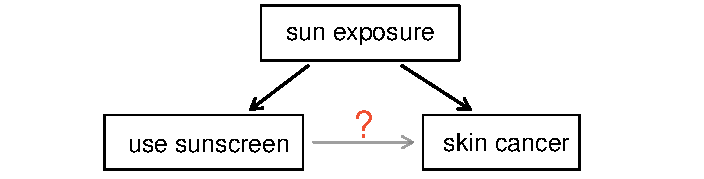
\includegraphics[height=1.0in]{01/figures/variables/sunCausesCancer}
\end{center}
It just so happens that if someone is exposed to the sun they also usually use sunscreen. Exposure to the sun is unaccounted for in the investigation, giving the incorrect impression that sunscreen causes skin cancer.

Sun exposure is what is called a \term{lurking variable}, which is a variable that is the true cause for change in the response. While one method to justify making causal conclusions from observational studies is to exhaust the search for lurking variables, there is no guarantee that all lurking variables can be examined or measured.

In the same way, the \data{possum} data set is an observational study with possible lurking variables of its own, and its data cannot easily be used to make causal conclusions.

\begin{exercise}
There appears to be a real difference in the proportion of possums that are male based on location. However, it is unreasonable to conclude that this is a causal relationship because the data is observational. Suggest at least one lurking variable that might be the true cause for the differences in \var{sex}. One lurking variable is listed in the footnote\footnote{Some genes can affect one gender more than the other. If the \resp{other} population has a gene that affects males more positively than females and this gene is less common in the \resp{Vic} population, this might explain the difference in gender ratio for each level of \var{pop}.}.
\end{exercise}

\subsection{Reducing bias in human experiments}
\label{biasInHumanExperiments}

Randomized experiments are the gold standard for data collection but do not ensure an unbiased perspective into the cause and effect relationships in all cases. Human studies are perfect examples where bias can unintentionally arise. Here we reconsider the sulphinpyrazone study, which was described in Section~\ref{basicExampleOfSulphinpyrazone}.

Researchers wanted to examine whether a drug called sulphinpyrazone would reduce the number of deaths after heart attacks. They designed an experiment because they wanted to draw causal conclusions about the drug's effect. Study volunteers\footnote{Human subjects are more often called \term{patients}, \term{volunteers}, or \term{study participants}.} were randomly placed into two study groups. One group, the \term{treatment group}, received the drug. The other group, called the \term{control group}, did not receive any drug treatment.

Put yourself in the place of a person in the study. If you are in the treatment group, you are given a fancy new drug that you anticipate will help you. On the other hand, a person in the other group doesn't receive the drug and sits idly, hoping her participation doesn't increase her risk of death. These perspectives suggest there are actually two effects: the one of interest is the effectiveness of the drug and the second is an emotional effect that is difficult to quantify.

Researchers aren't interested in this emotional effect, which might bias the study. To circumvent this problem, researchers do not want patients to know which group they are in. When researchers keep the patients in the dark about their treatment, the study is said to be \term{blind}. But there is one problem: if a patient doesn't receive a treatment, she will know she is in the control group. The solution to this problem is to give fake treatments to patients in the control group. A fake treatment is called a \term{placebo}, and an effective placebo is the key to making a study truly blind. A classic example of a placebo is a sugar pill that is made to look like the actual treatment pill. Often times, a placebo results in a slight but real improvement in patients. This often positive effect has been dubbed the \term{placebo effect}.

% Researchers aren�t interested in this emotional effect, which might bias the study, although it is not entirely obvious which way the bias would be. There are two methods to reduce or eliminate the bias. First, give the patients in the control group a fake treatment, which is called a placebo. Usually this is just a sugar pill that looks like the real drug. Then, for this placebo to eliminate this emotional effect, don�t tell any of the patients if they are receiving the real drug or the placebo so all are under the same emotional condition. In this setup, the study is said to be \term{blind} since no patients know their treatment. Findings suggest patients in control groups respond differently when the study is blinded to when it is not, and this effect  that the placebo is eliminating is aptly named the \term{placebo effect}.

The patients are not the only ones who should be blinded: doctors and researchers can accidentally bias a study. When a doctor knows a patient has been given the real treatment, she might inadvertently give that patient more attention or care than a patient that she knows is on the placebo. To guard against this bias (which again has been found to have a measurable effect in some instances), most modern studies employ a \term{double-blind} setup where doctors or researchers who interact with patients are, just like the patients, unaware of who is or is not receiving the treatment\footnote{There are always some researchers involved in the study who do know which patients are receiving which treatment. However, they do not have interactions with the patients and do not tell the blinded doctors who is receiving which treatment.}.

\subsection{Variability within data}
\label{variabilityWithinData}

The study examining the effect of sulphinpyrazone was double-blinded, and the results are summarized in Table~\ref{sulphinpyrazoneResults}. The variables have been called \var{group} and \var{outcome}. Do these results mean the drug was effective at reducing deaths? In the observed groups, a smaller proportion of individuals died in the treatment group than the control group (0.056 versus 0.081), however, it is unclear whether that difference is \emph{convincing evidence} that the drug is effective.
\begin{table}[ht]
\begin{center}
\begin{tabular}{l l cc rr}
& & \multicolumn{2}{c}{\var{outcome}} \\
  \cline{3-4}
		&			& 	\resp{lived} 	& \resp{died} & Total & \hspace{3mm}  \\ 
  \cline{2-5}
		&	\resp{treatment} 	& 692    		& 41   & 733  	 \\ 
  \raisebox{1.5ex}[0pt]{\var{group}}		&	\resp{control} 	& 682    		& 60     & 742	 \\ 
  \cline{2-5}
  		&	Total		& 1374	& 101	&  1475 \\
  \cline{2-5}
\end{tabular}
\end{center}
\vspace{-2mm}
\caption{Summary results for the sulphinpyrazone study.}
\label{sulphinpyrazoneResults}
\end{table}

\begin{example}{Suppose there had been only 45 deaths in the control group and still only 41 deaths in the treatment group. Would this be convincing evidence that the drug was effective?} \label{45PlaceboDeaths}
The proportion is still in favor of the drug (0.056 versus 0.061). However, this sample difference seems more likely to happen than 0.056 and 0.081. 
%A more definitive method will have to wait until later in the book. For now, it is worth noting data are random, so the statistics based on them will be random too. Sample data can only provide us with an estimate of the truth. 
It would actually be surprising if the sample proportions in each group were \emph{exactly} equal. When we collect data, there is usually a little bit of wiggle in the data. That is, the sample data only provides an \emph{estimate} of the truth.
\end{example}

Example~\exam{45PlaceboDeaths} is a reminder that the sample will not perfectly reflect the population. It is possible to see a small difference \emph{by chance}. Small differences in large samples can be important and meaningful but it is unclear when we should say that a difference is so large it was probably not due to chance. In Section~\ref{caseStudyOfSulphinpyrazone}, we evaluate whether Table~\ref{sulphinpyrazoneResults} shows convincing evidence that sulphinpyrazone is effective at reducing deaths or whether we remain unconvinced. %the difference of 2.5\% in the death rates was due to chance. %Chapter~\ref{foundationsForInference} provides a more general and rigorous framework to form conclusions based on data.

